\documentclass[a4paper]{article}
\title{Projectdossier VOP}
% Packages
\usepackage{fullpage}
\usepackage[dutch]{babel}
\usepackage[T1]{fontenc}
\usepackage[utf8]{inputenc}
\usepackage{hyperref}
\usepackage{graphicx}
\usepackage{epstopdf}
\usepackage{fancyhdr}
\usepackage{array}
\usepackage{amsmath}
\usepackage{multirow}
\usepackage{rotating}
\usepackage{wrapfig}
\usepackage{textcomp}
\usepackage{gensymb}
\usepackage{newunicodechar}
\usepackage{float}
\usepackage{siunitx}
\usepackage{amsthm}
\usepackage{lipsum}
\usepackage{ltxtable}

% Settings
\renewcommand{\arraystretch}{1.5}
\newcommand{\HRule}{\rule{\linewidth}{0.5mm}}
\newcommand{\specialcell}[2][c]{%
  \begin{tabular}[#1]{@{}c@{}}#2\end{tabular}}
\pagestyle{fancy}
\fancyhf{}
\renewcommand*{\headrulewidth}{0pt}
\fancyfoot[L]{Projectdossier VOP}
\fancyfoot[R]{\thepage}

% Custom commands
\newcommand{\studenten} {Tomas Bolckmans \\Thomas Clauwaert\\Aaron Mousavi\\Dwight Kerkhove\\Niels Verbeeck}
\newcommand{\begeleiders}{H. Naessens\\V. Ongenae\\P. Maenhaut} 
\newcommand{\titel}{Projectdossier VOP: Verkeerscentrum}
%\newcommand{\ondertitel}{}
\newcommand{\datum}{xx mei 2016}
\newcommand{\academiejaar}{2015-2016}

\newtheorem{stelling1}{Theorem}

\begin{document}

% Title page
\begin{titlepage}
\begin{center}

\includegraphics[height=4cm]{Images/Ugentlogo.eps}\\[.5cm]

Schakeljaar Master of Science in de\\
industriële wetenschappen: informatica\\
Academiejaar \academiejaar{}

\vfill

\HRule \\[0.4cm]
{\huge \bfseries \titel{}}\\[0.4cm]
\HRule \\[0.4cm]

%{\Large \ondertitel{}}\\[0.4cm]

Ingediend op \datum{}

\vfill
\begin{minipage}{0.49\textwidth}
\begin{flushleft}
\textbf{Studenten} verkeer 4\\
\studenten{}
\end{flushleft}
\end{minipage}
\begin{minipage}{0.49\textwidth}
\begin{flushright}
\textbf{Professoren}\\
\begeleiders{}\\
\end{flushright}
\end{minipage}

\end{center}
\end{titlepage}

\tableofcontents
\newpage

\section{Inleiding}
\label{sec:inleiding}
\lipsum[56]

\section{Statusverslag:}
\label{sec:statusverslag}
\lipsum[56]

Een duidelijk overzicht van welke features al dan
niet werden gerealiseerd (Vertrek hierbij van de backlogs en
geef voor elke feature aan in welke mate die beschikbaar is in
het eindproduct. Werd een feature slechts deels gerealiseerd,
geef dan ook aan welke beperkingen er zijn.

\section{Taakverdeling}
\label{sec:taakverdeling}

\section{Analyse}
\label{sec:analyse}

\section{Use cases}
\subsection{Globale domeinregels}

Wanneer er sprake is van \textbf{\textit{``providers''}} dan wordt hiermee de verzameling van geïmplementeerde providers bedoelt. Deze bestaan momenteel uit TomTom, Coyote, HereMaps, Google Maps, Bing Maps en Waze. Indien er een providerafhankelijke beslissing werd genomen dan zal dit gespecificeerd worden.

Een operator is altijd een gebruiker. Het verschil tussen beide valt nog nader te bespreken met de klant.

\textbf{DR Trajectinformatie}: een traject heeft ...

\textbf{DR Providers}:

\textbf{DR Filters}:

\textbf{DR Waze}: gegevens mogen niet ..

\newpage

\subsection{Voorbeeld}
\LTXtable{\textwidth}{Use-cases/Voorbeeld.tex}
\newpage

\subsection{Reistijd gegevens verzamelen}
\LTXtable{\textwidth}{Use-cases/GegevensVerzamelen.tex}
\newpage

\subsection{Trajectenoverzicht bekijken}
\LTXtable{\textwidth}{Use-cases/OverzichtBekijken.tex}
\newpage

\subsection{Trajectdetail bekijken}
\LTXtable{\textwidth}{Use-cases/DetailBekijken.tex}
\newpage

\subsection{Trajectmap bekijken}
\LTXtable{\textwidth}{Use-cases/MapBekijken.tex}
\newpage

\subsection{Providerdata vergelijken}
\LTXtable{\textwidth}{Use-cases/DataVergelijken.tex}
\newpage

\subsection{Traject wijzigen}
\LTXtable{\textwidth}{Use-cases/TrajectWijzigen.tex}
\newpage

\subsection{Traject toevoegen}
\LTXtable{\textwidth}{Use-cases/TrajectToevoegen.tex}
\newpage

\subsection{Traject verwijderen}
\LTXtable{\textwidth}{Use-cases/TrajectVerwijderen.tex}
\newpage

\subsection{Statuspagina bekijken}
\LTXtable{\textwidth}{Use-cases/LogpaginaBekijken.tex}
\newpage

\subsection{Infopagina's bekijken}
\LTXtable{\textwidth}{Use-cases/InfoPaginasBekijken.tex}
\newpage

\subsection{Dashboard bekijken}
\LTXtable{\textwidth}{Use-cases/DashboardBekijken.tex}
\newpage

\subsection{Traject gegevens met reistijden aanbieden}
\LTXtable{\textwidth}{Use-cases/ReistijdenAanbieden.tex}
\newpage

\subsection{POI gegevens verzamelen}
\LTXtable{\textwidth}{Use-cases/POIGegevens.tex}
\newpage

\subsection{Weer gegevens verzamelen}
\LTXtable{\textwidth}{Use-cases/WeerGegevens.tex}
\newpage

\subsection{Parkeer \& bord gegevens verzamelen}
\LTXtable{\textwidth}{Use-cases/ParkeerGegevens.tex}
\newpage

\section{Non-Functional Requirements (NFRs)}
\subsection{Voorbeeld}
\LTXtable{\textwidth}{NFRs/Voorbeeld.tex}

\subsection{Look \& Feel Requirements}
\LTXtable{\textwidth}{NFRs/Huisstijl.tex}

\subsection{Look \& Feel Requirements}
\LTXtable{\textwidth}{NFRs/VisueelOverzichtelijk.tex}

\subsection{Usability \& Humanity Requirements}
\LTXtable{\textwidth}{NFRs/Responsive.tex}

\subsection{Operationele \& omgevingsrequirementss}
\LTXtable{\textwidth}{NFRs/Productie.tex}

\subsection{Wettelijke requirements}
\LTXtable{\textwidth}{NFRs/Afscherming.tex}


Under review:


- Security Requirements: Hoe wordt admin stuff geregeld?

- Security Requirements: app mag niet exploitbaar zijn




\section{Mockups}

Dashboard mockup + Statuspagina mockup

\section{Diagrammen}
met toelichting

\begin{figure}[H]
\centering
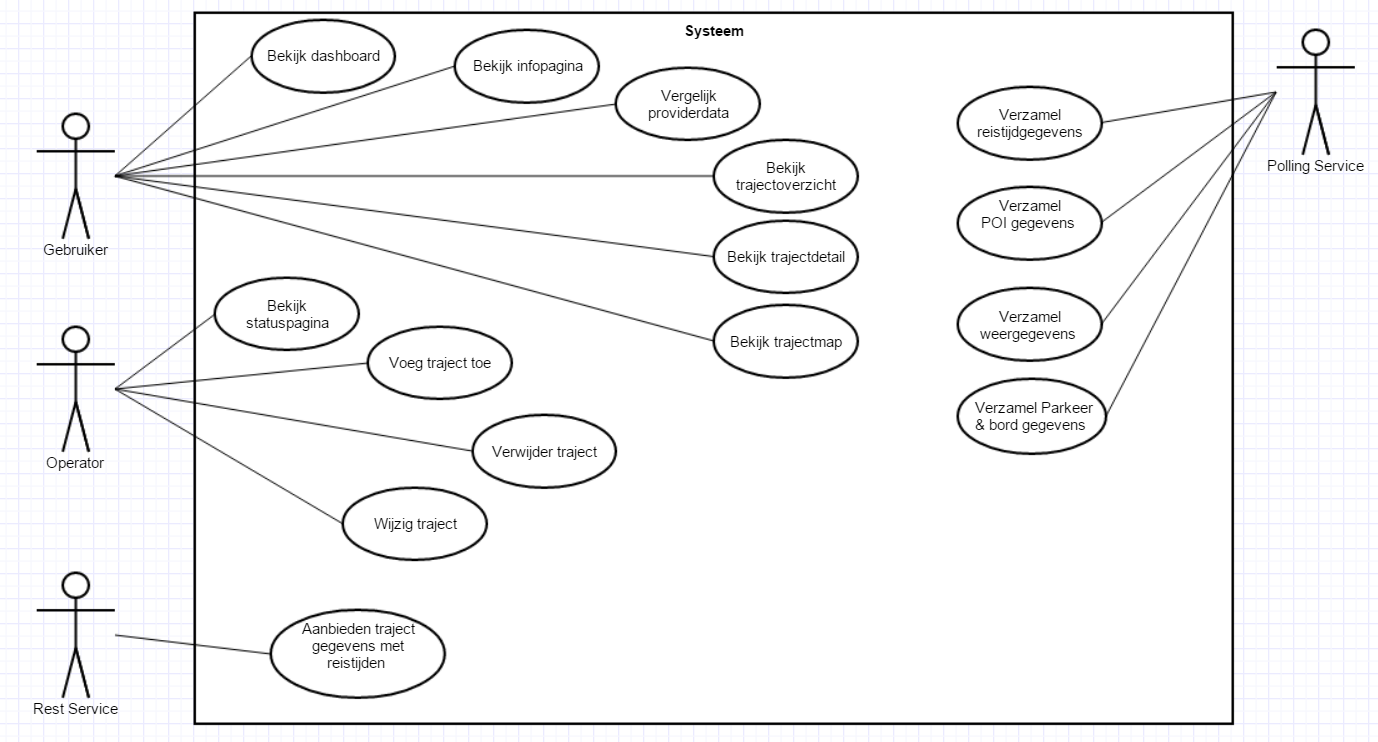
\includegraphics[width=\textwidth]{Images/usecasediagramv3.png}\\
\caption{Use Case Diagram}
\end{figure}

\section{Vragen en antwoorden}



\section{Kwaliteitscontrole}
\label{sec:kwaliteitscontrole}

(methodologie m.b.t. testen);
\section{Gebruikershandleiding}
\label{sec:gebruikershandleiding}

een gebruikershandleiding voor de verschillende applicaties;
\section{Installatiehandleiding}
\label{sec:installatiehandleiding}
installatiehandleiding.

De schriftelijke neerslag van jullie prestaties bestaat uit een
geniete bundel met alle documentatie op papier.
Spendeer voldoende tijd voor het opstellen en nalezen van de
documentatie. We verwachten van elk team een netjes afgewerkt
en coherent geheel. Besteed dus de nodige zorg aan taal en stijl.

\section{Productbacklog}
\label{sec:productbacklog}
\begin{table}[H]
\centering
\begin{tabular}{|l|c|c|c|} 
\hline
\textbf{Use case} & \textbf{Must have} & \textbf{Nice to have}  & \textbf{Weging (uur)}\\ \hline \hline
Verzamel reistijdgegevens & 1 & & 5000 \\ \hline 
Bekijk trajectoverzicht & 2 & & 5000 \\ \hline 
Bekijk trajectdetail & 2 & & 5000 \\ \hline 
Bekijk trajectmap & 3 & & 5000 \\ \hline 
Vergelijk providerdata & 4 & & 5000 \\ \hline
Wijzig traject & & 12 & 5000 \\ \hline
Voeg traject toe & & 14 & 5000 \\ \hline
Verwijder traject & & 14 & 5000 \\ \hline
Bekijk statuspagina & & 12 & 5000 \\ \hline 
Bekijk infopagina's & & 13 & 5000 \\ \hline 
Bekijk dashboard & & 13 & 5000 \\ \hline 
Aanbieden trajectgegevens met reistijden & & 11 & 5000 \\ \hline
Verzamel POI gegevens & & 16 & 5000 \\ \hline
Verzamel Weergegevens & & 16 & 5000 \\ \hline
Verzamel Parkeer \& bord gegevens & & 16 & 5000 \\ \hline
\end{tabular}
\caption{Productbacklog \label{productbacklog}}
\end{table}

\newpage

\listoffigures
\listoftables

\end{document}